
\subsection{The Control Flow graph}\label{abstrCntrFlow}
As we  already stated we assume that loops in method bodies are  \textit{annotated} with appropriate invariants. 
Related works like in \cite{WildmoserN-ESOP05} use different approach where they infer loop invariants. Anyways inferring invariants is not decidable. 
Rather we propose the scheme where the programmer writes the invariants during the program development  
and on compilation time they are compiled in BCL. Under the assumption for invariant presence we may ``cut'' the control flow graph at every program point
where an invariant must hold and ``place'' there the invariant. Here we describe which are the points in the bytecode which are "cut". This needs the introduction
of several definitions.
     
 A method body is an array of bytecode instructions that is denoted with $i$ and the $k-th$ instruction
 in the bytecode is  denoted with $i_{k}$.
 We denote by $\Gamma  = ( \Omega, \ll)$ the control flow graph of a
bytecode $\Pi$ where the set of nodes $\Omega$ is the set of
blocks. Using standard terminology \cite{ARUCom1986}, a
basic block is a code segment that has no unconditional jump or
conditional branch statements except for possibly the last
statement, and none of its statements, except possibly the first,
is a target of any jump or branch statement. 
 We denote a block starting at instruction  $i_{j}$ with $\blockm{j}$. Let's have 
the bytecode $\Pi$ and the set of its blocks be $\wp$. The execution relation ( $\blockm{j} \execRel \blockm{k}$ ) states that block
$ \blockm{k}$ may be executed immediately after $\blockm{j}$ in some execution path of the method. 
The  definition is given at \ref{execRel}

\begin{defn}[Execution relation between blocks]\label{execRel}
\begin{tabbing}
\\Let \=  have \= the block $\blockm{j}$ such that  it ends with instruction \\ 
$\tt{i_{k}}$ and it is not a return instruction\\
\>  if $\tt{i_{k}}$ = \texttt{if\_cond n} then   $\blockm{j} \execRel \blockm{n}$ and $\blockm{j} \execRel  \blockm{k+1} $ \\
\>  if $\tt{i_{k}}$ = \texttt{goto n} then $\blockm{j} \execRel \blockm{n}$ \\
\>  if $\tt{i_{k}}$ = \texttt{athrow} then $\blockm{j} \execRel \blockm{n}$ for all \texttt{n}, such \\
\> \> that $\blockm{n}$ is the first\\
\> \> block of an exception handler that protects $\tt{i_{k}}$ \\
\>  if $\tt{i_{k}}$ = \texttt{jsr n} then $\blockm{j} \execRel \blockm{n}$ \\
\>  if  $\tt{i_{k}}$ = \texttt{ret n} then  $ \blockm{j} \execRel \blockm{s}$\\
\> \> for all s that are indexes of instruction following \\
\> \> a \texttt{jsr} to the subroutine that ends with $\tt{i_{k}}$ instruction\\
\>  else $\blockm{j}  \execRel   \blockm{k+1}$
\end{tabbing}
\end{defn}

We say that there exists a path between $\blockm{i}$ and $\blockm{j}$ and we note it with  $\pathm{i}{j}$, if there exists blocks 
$\blockm{s_{1}}... \blockm{s_{n}}$ such that $\blockm{i} \execRel \blockm{s_{1}} \execRel \blockm{s_{2}}... \blockm{s_{n}} \execRel  \blockm{j}$
\begin{defn}[Loop Definition]
\label{defLoop}
Let's have a well formed program $\Pi$. We say that $\blockm{s}$ is the entry block of loop $l$ in $\Pi$ and $\blockm{e}$ is the end block of $l$ if:
\begin{itemize}
\item every path in the control flow graph starting at the entry block $\blockm{entry}$ (i.e. the one
 that starts with the entry instruction) of $\Pi$ and that reaches $\blockm{e}$, passes through  $\blockm{s}$ 
  i.e.$ \blockm{entry} \execRel^{*}  \blockm{s} \execRel^{*} \blockm{e}$
\item $\blockm{e} \execRel \blockm{s}$
\end{itemize}
\end{defn}


\subsection{Acyclic control flow graph} \label{graph}
We consider the acyclic graph $\Gamma^A = ( \Omega, \execRel^A)$ obtained from the control flow graph 
$\Gamma  = ( \Omega, \execRel)$ of a well formed bytecode $ \Pi $. The set of nodes $\Omega$ is the set of  blocks in the 
program and the relation  $\execRel^A$ is a subset of the  execution relation $\execRel$.
\begin{defn}[Acyclic Execution relation]
\label{acyclicExRel}
Let's have the well formed bytecode program $\Pi$ and let have in $\Pi$ the two blocks  $\blockm{i} $ and   $\blockm{j}$. We say 
that $\blockm{i} \execRel^A \blockm{j}$ iff
\begin{itemize}
\item $\blockm{i} \execRel \blockm{j}$
\item and block $\blockm{i}$ and block $\blockm{j}$ are not the end and the entry blocks respectively of the same loop, see loop definition~\ref{defLoop}.
\end{itemize}
\end{defn}

Both the cyclic and acyclic graphs of the bytecode of method \texttt{half} at Fig.~\ref{halfBC} is at Fig. ~\ref{blockBC}. Blocks are represented by boxes. Black arrows stand for relation $\execRel^A$. Dashed arrows represent relation $\execRel$.

\begin{figure}[p]
\begin{center}
\begin{tabular}{rl}
 0 & iconst\_0\\ 
 1 & istore\_2\\
 2 & iload\_1\\
 3 & istore\_3\\%[-2mm]
 4 & goto 13 (+9)\\%[-2mm]
 7 & iinc 2 by 1\\%[-2mm]
10 & iinc 1 by 254\\%[-2mm]
13 & iload\_1\\%[-2mm]
14 & iconst\_1\\%[-2mm]
15 & if\_icmpgt 7 (-8)\\%[-2mm]
18 & iload\_2\\%[-2mm]
19 & ireturn\\%[-2mm]
\end{tabular}
\end{center}
\caption{the bytecode of method \texttt{half}}
\label{halfBC}
\end{figure}

\begin{figure}[p]
\begin{center}
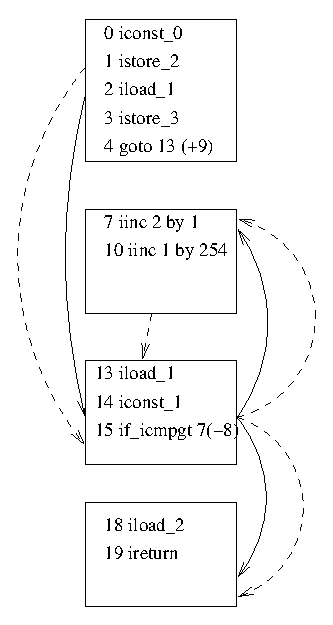
\epsfig{file=graph.eps}
\end{center}
\caption{bytecode blocks of bytecode at Figure ~\ref{halfBC}}
\label{blockBC}
\end{figure}

Now a path in $\Gamma^A$  is a list of blocks between which is established a relation $\execRel^A$ and that starts at the entry point instruction and whose last block is a block that does not have next block.

